% The cycle of Theorem 6.1: the paths and the pool vertices joining them.
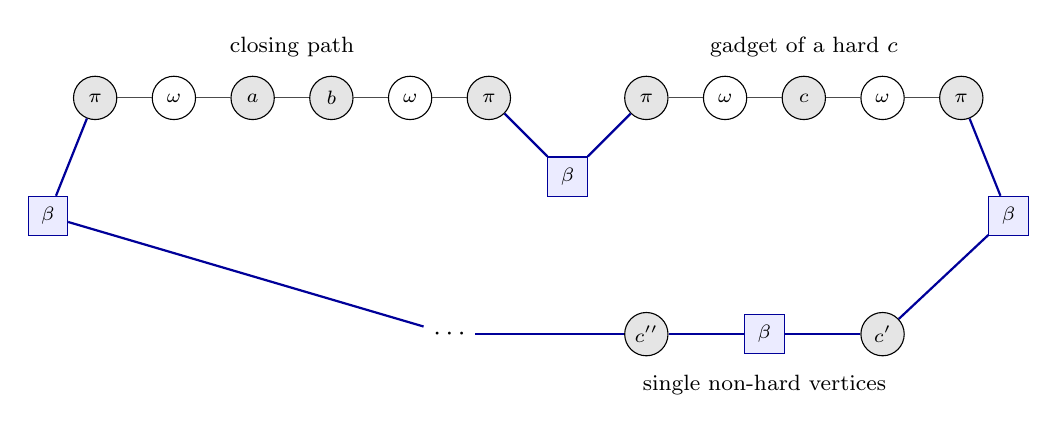
\begin{tikzpicture}[
  od/.style={circle, draw=black, fill=black!10, inner sep=1.5pt, minimum size=5.5mm, font=\scriptsize},
  ev/.style={circle, draw=black, fill=white, inner sep=1.5pt, minimum size=5.5mm, font=\scriptsize},
  pl/.style={rectangle, draw=blue!60!black, fill=blue!8, inner sep=2pt, minimum size=5mm, font=\scriptsize},
  e/.style={black!70}, j/.style={blue!60!black, thick}]
% closing path
\node[od] (p1) at (0,0) {$\pi$};
\node[ev] (w1) at (1,0) {$\omega$};
\node[od] (a) at (2,0) {$a$};
\node[od] (b) at (3,0) {$b$};
\node[ev] (w2) at (4,0) {$\omega$};
\node[od] (p2) at (5,0) {$\pi$};
\draw[e] (p1)--(w1)--(a)--(b)--(w2)--(p2);
\node[font=\footnotesize] at (2.5,0.65) {closing path};
% pool vertex
\node[pl] (q1) at (6,-1) {$\beta$};
% gadget
\node[od] (g1) at (7,0) {$\pi$};
\node[ev] (gw1) at (8,0) {$\omega$};
\node[od] (c) at (9,0) {$c$};
\node[ev] (gw2) at (10,0) {$\omega$};
\node[od] (g2) at (11,0) {$\pi$};
\draw[e] (g1)--(gw1)--(c)--(gw2)--(g2);
\node[font=\footnotesize] at (9,0.65) {gadget of a hard $c$};
\node[pl] (q2) at (11.6,-1.5) {$\beta$};
% singletons
\node[od] (s1) at (10,-3) {$c'$};
\node[pl] (q3) at (8.5,-3) {$\beta$};
\node[od] (s2) at (7,-3) {$c''$};
\node[font=\footnotesize] at (8.5,-3.65) {single non-hard vertices};
\node (dots) at (4.5,-3) {$\cdots$};
\node[pl] (q4) at (-0.6,-1.5) {$\beta$};
\draw[j] (p2) -- (q1) -- (g1);
\draw[j] (g2) -- (q2) -- (s1);
\draw[j] (s1) -- (q3) -- (s2);
\draw[j] (s2) -- (dots);
\draw[j] (dots) -- (q4) -- (p1);
\end{tikzpicture}
